\cotefile{85}
\scanpage{44}

Sous-groupes finis de \deleted{\unsure{Aut}} $\underline{\mathrm{Aut}}_{\!X}\deleted{(X)}=\mathbb A$ ($X$ droite projective sur corps \unsure{alg} \inserted{de car.~$0$})

\unsure{1.)|1)} Sous-groupes $\Gamma^{+},\Gamma\subset\mathbb A$ qui sont des formes de $\unsure{A_4|\mathcal A_4|\mathfrak A_4}$ ou $\unsure{\mathfrak S_4|\mathcal S_4}$. Se correspondent biunivoquement

\[
\Gamma^{+}\longmapsto\Gamma=\mathrm{Norm}_{\unsure{G|A|\mathbb A}}(\Gamma^{+})\qquad
\Gamma^{+}=[\Gamma,\Gamma]
\]

\uline{NB} $\mathrm{Aut}(A_4)\xleftarrow{\sim}\mathrm{Aut}(\mathfrak S_4)\xleftarrow{\sim}\mathfrak S_4$ On aura : la cat. des ensembles à $4$ él., celle des formes de $A_4$, celle des formes de $\mathfrak S_4$, sont équivalentes

\diagram{\begin{tikzcd}[ampersand replacement=\&,column sep=small]
 F(\mathfrak S_4)\arrow[rr,dash,"\sim"]\arrow[dr,dash,"\sim"'] \& \& F(A_4)\arrow[dl,dash,"\sim"]\ {\deleted{\unsure{(Ens)_4}}} \\
 \& (\mathrm{Ens})_4 \&
\end{tikzcd}}

\[
\begin{aligned}
E\in(\mathrm{Ens})_4,\ &\longmapsto\Gamma=\mathfrak S_E,\ \Gamma^{+}=\mathfrak S_E^{+}\\
\Gamma^{+}\in F(A_4)&\longmapsto\Gamma=\mathrm{Aut}(\Gamma^{+}),\ \text{$E\unsure{=}$ ens des ss-gpes d'indice $4$}\\
&\hspace{6em}\text{(d'ordre $3$) de $\Gamma^{+}$}\\
\Gamma\in F(\mathfrak S_4)&\longmapsto\Gamma^{+}=[\Gamma,\Gamma],\quad E=\text{ens des ss-gpes $\inserted{\gamma}$ d'ordre $6$ (indice $4$)}\\
&\hspace{3em}\text{de $\Gamma$}\simeq\text{ ens des ss-gpes}\\
&\hspace{4em}\gamma^{+}\text{ d'ordre $3$ de $\Gamma$}\\
&\quad[\,\gamma^{+}=[\gamma,\gamma],\ \gamma=\mathrm{Norm}_{\Gamma}(\gamma^{+})\,]
\end{aligned}
\]

Donc sur schéma $S$

\[
\mathrm{Rev}_4(S)\simeq F(S,\mathfrak S_4)\simeq F(S,A_4)
\simeq\mathrm{Tors}(\mathfrak S_{4S})\simeq\text{\uline{Cubes orientés sur $S$}}
\]

\deleted{\unsure{$\simeq$}} \uline{Re NB} En car $0$ (\unsure{inutile} ?) Si $\Gamma^{+}$ ou $\Gamma\subset\deleted{X,\ \text{alors}}\inserted{G=\underline{\mathrm{Aut}}_{\!X}},$ alors [tout autom de $\mathbb A$ est int, $\mathbb A\mathrel{\overset{\mathrm{int}}{\simeq}}\mathrm{Aut}(\mathbb A),$ et] tout autom de $(\mathbb A,\Gamma^{+})$ ou $(\mathbb A,\Gamma)$ qui normalise $\Gamma^{+}$ ou $\Gamma$ provient de $\Gamma$ : $\Gamma\xrightarrow{\sim}\underline{\mathrm{Aut}}_{(X,\Gamma)},\ \Gamma\simeq\underline{\mathrm{Aut}}_{(X,\Gamma^{+})}$

Donc la cat. des couples $(\Gamma,X)$ $(\Gamma^{+},X)$ est équivalente à celle des torseurs sous $\mathfrak S_{4S}$, i.e. aux cat. précédentes -- donc aussi à celle des \uline{cubes orientés} sur $S$, ou celle des \uline{tétraèdres} (pas \deleted{\unsure{néce.}} orientés) sur $S$. Dans ce

% archive sheet number: 43
\scanpage{45}

dictionnaire, $\Gamma$ s'interprète comme le \deleted{\unsure{tétr}} Groupe des autom du tétraèdre, ou du cube orienté, $\Gamma^{+}$ comme le gpe des autom \uline{orientés} du tétraèdre (ou celui des automorphismes ``biorientés'' du cube) \ldots

2. On s'intéresse \deleted{plus \unsure{m}} aux systèmes $\deleted{\unsure{(H\subset G,)}}\inserted{(\mathbb A,\deleted{\unsure{G}}\mathbb H,}\rho,\rho',\rho'')$ où $\rho,\rho',\rho''$ sont des sections \deleted{qui} \inserted{de} $G$, \inserted{telles que $\rho\rho'\rho''=1$} qui engendrent un ss-gpe fini $\mathbb H$, non abélien ni diédral (i.e. $\simeq \unsure{A_4|\mathcal A_4|\mathfrak A_4},\unsure{\mathfrak S_4|\mathcal S_4}$ ou $A_5$) -- Donc $H$ sera une forme splittée de l'un de ces gpes (mais $X$ \inserted{ou $G$} ne sera pas splitté pour autant --)

% slanted
\margin{\uline{NB} $\mathbb H$ résulte de $\rho,\rho',\rho''$, et $\rho''$ résulte de $\rho,\rho'$ (et $\rho$ de $\rho',\rho''$, $\rho'$ de $\rho'',\rho\ldots$)}

\unsure{On} \unsure{peut} dire aussi (sur base $S$ connexe) qu'à la donnée $\rho,\rho',\rho''$ correspond un tétraèdre \inserted{comb.} \unsure{resp.} un cube orienté \inserted{comb.} (\unsure{resp|ou} un biicosaèdre comb., cf plus bas) qui définit $X$ (modulo grain de sel du cas icosaédral \ldots), qu'on peut oublier. Et on se propose de trouver les syst. de trois gén. $\rho,\rho',\rho''$ du gpe \deleted{\unsure{$H$}} ``abstrait'' $H$ des autom orientés du \deleted{cube} tétraèdre, ou du cube \ldots\ \deleted{\unsure{laissant|laissons} l'icos-}

Notons qu'un autom de $(G,\rho,\rho',\rho'')$ est un autom de $(G,H)$ qui commute à $\rho,\rho',\rho''$ i.e. à $H$, donc \deleted{est} trivial (car le centr. de $H$ est réduit au gpe unité). Donc on a catégorie \uline{rigide} : ces objets sont définis à isom. \uline{unique} près, pour la classe d'isom. donnée.

% archive sheet number: 44
\scanpage{46}

\uline{Rmq} Comme premier invariant d'un système $\rho,\rho',\rho''$, il y a \unsure{les|le} \inserted{triplet des} \uline{ordres} $(\unsure{\nu|v},\nu',\nu'')$ de $\rho,\rho',\rho''$. Les op. de $\unsure{\mathfrak S_3|\mathcal S_3}$ sur $H^3$ correspondent \unsure{évidemment|évidemt} aux op. de $\mathfrak S_3$ sur $\mathbb N^3$. Notons $\nu,\nu',\nu''\geq 2$ et

\diagram{$\begin{array}{c@{\ }l}
\begin{array}{c}\mathrm I\\\mathrm{II}\\\mathrm{III}\end{array}&
\left\{\begin{array}{ll}
2\leq\nu,\nu',\nu''\leq3&\text{cas }\unsure{A_4|\mathcal A_4|\mathfrak A_4}\\
2\leq\nu,\nu',\nu''\leq4&\text{cas }\mathfrak S_4\\
2\leq\nu,\nu',\nu''\leq5&\text{cas }A_5
\end{array}\right.
\end{array}$}

On verra que dans le premier cas, \deleted{\unsure{les|le}} triplet contient \deleted{\unsure{contient}} $3$, dans le deuxième il contient $4$, dans le troisième il contient $5$ -- donc le triplet numérique implique déjà dans lequel des cas I, II, III on se trouve (\deleted{\unsure{en reg|en regardant}} suivant que son sup est $3,4$ ou $5$). Dans les cas I II, on voit que $(\rho,\rho',\rho'')$ est déterminé mod iso par son caractère numérique. Dans le cas icosaédr. III, il n'en est plus tout à fait ainsi (pas même pour l'équivalence modulo $\mathfrak S_5$ opérant) -- il faut préciser un peu le critère numérique [en distinguant les deux classes de conjugaison d'él. d'ordre $5$ dans $A_5$ \ldots]

\deleted{3) Cas de $A_4$.}

\deleted{\uline{Théorème} Soit $\Pi$ un tétraèdre \inserted{comb.} orienté, $\unsure{\mathbb H|H}$ le gpe de ses automorphismes \inserted{(orientés)}. À tt sommet $s\in S$ de $\Pi$ est associé un $\rho_s\in H$, él. d'ordre $3$ et on trouve ainsi une bijection de $S$ \deleted{\unsure{dans}} l'ens. des \inserted{$8$} éléments d'ordre $3$ de $H$, soit $H_3^+$ son image, de sorte}

% archive sheet number: 45
\scanpage{47}

Notons que si $H$ est un gpe abstrait, $\mathrm{Tr}(H)$ l'ens des $(\rho,\rho',\rho'')\in H^3$ tels que $\rho\rho'\rho''=1$, le groupe $\unsure{\mathfrak S_3|\mathcal S_3}$ opère dedans de façon évidente, l'orbite de $(\rho,\rho',\rho'')$ \deleted{$(\rho,\rho',\rho'')\ \unsure{\text{et}}\ (\rho',\rho'',\unsure{\rho''|\rho})$} étant formée de

\[
(\rho,\rho',\rho'')\quad(\rho',\rho'',\rho)\quad(\rho'',\rho,\rho')\quad
(\rho''{}^{-1},\rho'{}^{-1},\rho^{-1})\quad
(\rho'{}^{-1},\rho^{-1},\rho''{}^{-1})\quad
(\rho^{-1},\rho''{}^{-1},\rho'{}^{-1})
\]

De cette façon, le gpe $\mathfrak S_3$ opère sur la cat. des ``groupes pythagoriciens avec présentation de Schwartz'' ou simplement Systèmes de Schwartz. On est intéressé à tenir compte de cette opération, et notamment déterminer quels sont les transformés \inserted{(par op. de $\mathfrak S_3$)} d'un $(H,\rho,\rho',\rho'')$ qui lui sont isom. \deleted{\unsure{et}}

\uline{Rmq} La notion d'isom qui nous intéresse est celle définie par le sch. en gpes ambiant $A$, ce qui s'explicite en \unsure{terme|termes} élémentaire ainsi :

a) Cas $\unsure{A_4|\mathcal A_4|\mathfrak A_4}$ : isomorphie par op. de $\mathfrak S_4$ \inserted{sur $A_4$} (\uuline{pas} $A_4$) On peut néanmoins se proposer de faire aussi la classification \uline{plus fine} \deleted{\unsure{du|dans}} d'op. de $A_4$.

b) Cas $\mathfrak S_4$ : isom par autom. int.

c) Cas $A_5$ : isom par autom. int. Il y a une classification moins fine, modulo autom. de $\mathfrak S_5$ sur $A_5$, qui donne ``moitié moins'' de classes d'isomorphie.

% archive sheet number: 46
\scanpage{48}

\deleted{que $H_3^{-}=H_3\setminus H_3^{+}$ est l'ens des $(\rho_s^{-1})_{s\in S}$, ou encore l'ens des $\rho_f$ ($f\in F$ ens des faces) \deleted{Noter que si $s,f$ st opposés}}

\margin{\uline{NB} si $s,f$ opposés, on a : $\rho_f=\rho_s^{-1}$}

\deleted{a) Pour toute \deleted{\unsure{couple}} \inserted{arête} $\{s,t\}$ de $\Pi$, le triple}

\[
\deleted{(\rho_t^{-1},\rho_s,\rho_t^{-1}\rho_s)}
\]

\deleted{engendre $H$, et est de type numérique $(3,3,2)$ Les \inserted{trois} él. d'ordre $2$ de $H$ étant identifiés aux \deleted{couples} \inserted{paires} d'arêtes ``opposées'' de $\Pi$ (comme \deleted{symétries} \inserted{\unsure{rotation complète|rotation compl.|rotations d'angle $\pi$}} p.r. à l'axe joignant leurs milieux)}

3. De façon générale, si $\Pi$ est un polyèdre comb. \inserted{régulier} \deleted{\unsure{orienté}} \inserted{\uline{orientable}}, et $H=\mathrm{Aut}^{+}(\Pi)$, on \deleted{\unsure{trouve}} associe à tte \deleted{\unsure{$f$}} \unsure{en|ou} tt $\varphi\in\mathrm{Fac}(\Pi)=S\amalg A\amalg F$, un op. $\rho_\varphi\in H$ \inserted{(en \uline{utilisant l'orientation})}, de sorte que pour tt \uline{repère} \inserted{\uline{direct}} $r=(s,a,f)$, le triple

\[
\Sigma_r=(\rho_f,\rho_s,\rho_a)\in H^3
\]

\margin{\uline{NB} $\Sigma_r$ ne dépend pas du choix préalable d'une orientation car $r$ en définit une.}

satisfasse $\rho_f\rho_s\rho_a=1$ (\uline{NB} $\rho_f\rho_s=\rho_a$ et $\rho_a^2=1$) ou encore $\rho_s\rho_a\rho_f=1$. On note que tous ces systèmes de générateurs sont conjugués sous $\mathrm{Aut}(\Pi)$,

\deleted{mais pas néc$^{\mathrm t}$ sous $H=\mathrm{Aut}^{+}(\Pi)$ car il faut distinguer \deleted{\unsure{$\rho$|les}} $\Sigma_r$ suivant que $r$ appartient à l'une ou l'autre orientation de $\Pi$. \deleted{\unsure{On est}} La question est donc quand il est vrai que $\Sigma_r$ et $\Sigma_{r'}$ conjugués sous $H$, avec $r,r'$ d'orientations opposées, p.ex.}

Si on prenait l'orientation opposée, on aurait $\rho_f^{-1}\ \rho_s^{-1}\ \rho_a^{-1}=\rho_a$ au lieu de $\rho_f,\rho_s,\rho_a$, on trouve

% archive sheet number: 47
\scanpage{49}

d'autres systèmes de gén.

\[
\Sigma_{r'}=(\rho_f^{-1},\rho_s^{-1},\rho_a=\rho_{\unsure{a|r}}^{-1})
\]

associés aux repères $r'=(s,a,f)$ \uline{indirects}
Les $\Sigma_{r'}$ sont conjugués entre eux sous $H$, et les $\Sigma_r$ et $\Sigma_{r'}$ sont conjugués sous $\mathrm{Aut}\,\Pi$, mais pas néc. sous $H=\mathrm{Aut}^{+}(\Pi)$ -- par exemple parce qu'il se peut que les $\rho_s$ et $\rho_s^{-1}$ (ou $\rho_f$ et $\rho_f^{-1}$) ne soient pas conjugués (cf icosaèdre).

\uline{Systèmes de Schwartz} \uline{canoniques} et \uline{anticanoniques} \unsure{associé|associés} au polyèdre régulier orienté.

Quand a-t-on

\[
\Sigma_{r_1}=\Sigma_{r_2}
\]

($r_1$ et $r_2$ \deleted{directs)} repères donnés) -- disons avec $=$ orientation, i.e.

\[
\rho_{s_1}=\rho_{s_2},\inserted{\text{et}}\ \rho_{f_1}=\rho_{f_2},\quad \rho_{a_1}=\rho_{a_2}
\]

\deleted{Il semble} Posons $r_2=g\cdot r_1$ ($g\in\mathrm{Aut}\,\Pi$ bien déterminé) alors

\[
\Sigma_{r_2}=g\cdot\Sigma_{r_1}=
(\mathrm{int}(g)\rho,\mathrm{int}\,g\rho',\mathrm{int}(g)\rho'')
\]

si $\Sigma_{r_1}=(\rho,\rho',\rho'')$. Donc $\Sigma_{r_2}=\Sigma_{r_1}$ \unsure{sss|ssi} $g$ appartient au \deleted{\unsure{centre}} \inserted{commutant} $\unsure{Z|3|\mathfrak Z}$ de $\mathrm{Aut}^{+}\Pi$ \inserted{dans $\mathrm{Aut}\,\Pi$}. Dans les cas où $\mathrm{Aut}\,\Pi=Z\cdot\mathrm{Aut}^{\unsure{+|\epsilon}}(\Pi)$ \inserted{(cas des II et III)}, on voit donc que \deleted{\unsure{$\Sigma_{r_1}$ et $\Sigma_{r}$}} tous les $\Sigma_r$ conjugués par $\mathrm{Aut}^{+}(\Pi)$ (pour les $r$ directs et inverses)

% archive sheet number: 48
\scanpage{50}

\uline{Proposition} Soit $\Pi$ un tétraèdre orienté, $R$ $(R^{+})$ l'ens de ses repères (\inserted{resp.} directs), $S,A,F$ l'ens des ses sommets, \deleted{\unsure{a}}arêtes, faces -- d'où $\rho_s,\rho_a,\rho_f$ si $s\in S$, $a\in A$, $f\in F$. \deleted{Soit} $\Phi=\underset{\inserted{4}}S\amalg\underset{\inserted{6}}A\amalg\underset{\inserted{4}}F$ l'ens des facettes

\deleted{a) Les applic$^{\mathrm{ns}}$ $s\unsure{\to|\mathord{-}}\rho_s$,}

a) L'application $\varphi\unsure{\longrightarrow|\mathord{-}|\mapsto}\rho_{\unsure{p|\varphi}}$ de $S\amalg F$ dans $H=\mathrm{Aut}^{+}\Pi$ est injective, et son image est l'ens des $8$ él. d'ordre $3$ de $H$. De plus, si $s\in S$, $f\in F$ sont opposés, on a \inserted{$\rho_s\rho_f=\rho_f\rho_s=1$}

b) L'application $a\longmapsto\rho_a$ de $A$ dans $H$ induit une application de degré $2$ de $A$ dans \inserted{(sur)} l'ens $ {}_3H$ des él. d'ordre $3$ de $H$ [\uline{NB} deux arêtes sont dites opposées si elles ont $=$ image, \deleted{\unsure{en}} qui signifie aussi que ce sont des parties disjointes de $S$, ou de $F$\unsure{]|.}

c) L'application $r\unsure{\longrightarrow|\mathord{-}|\mapsto}\Sigma_r$ de $R$ dans l'ens des syst. de Schwartz de $H$ est injective [en effet le commutant de $H$ dans $\inserted{\widetilde H=}\mathrm{Aut}(\Pi)$ est $1$] l'image forme donc une classe sous $\widetilde H$ (\deleted{qui} c'est un torseur sous $\widetilde H$) et deux classes sous $H$, de type numérique $(3,3,2)$.

\margin{$24=12+12$ syst. de Schwartz}

% slanted
\margin{[celà fait $72=36+36$ en transformant par $\unsure{\mathfrak S_3|\mathcal S_3}$, deux paquets de $36$ syst. de Schwartz, \deleted{\unsure{chacun des} paquets de $72$ est stable par $\mathfrak S_3$ \unsure{et} \illegible{1}} stables sous $\mathfrak S_3\times H$}

d) Si on a un syst. de Schwartz canonique $(\rho_f,\unsure{\rho'_s|\rho_s},\rho'_a)$ \inserted{[ou anticanonique $(\rho'_{f},\rho'_{s},\rho'_{a})$]}, les $6$ systèmes qu'il engendre, par \deleted{\unsure{son|action}} \deleted{\unsure{$\rho_f,\rho_s,\rho_a$}} \deleted{$(\rho,\rho',\rho'')\ (\rho'',\rho,\rho')$} \deleted{\unsure{cla}} gpent donc $2$ par $2$ suivant des \deleted{$(\rho,\rho',\rho''),(\rho',\rho'',\rho)(\rho'',\rho,\rho')($} types numériques égaux, ceux qui sont de type numérique comme

\[
(\rho_f,\rho_s,\rho_a),\quad
(\underset{\inserted{\rho''_{f'}}}{\rho_s^{-1}},
 \underset{\inserted{\rho''_{s'}}}{\rho_f^{-1}},
 \underset{\inserted{\rho''_{a'}}}{\rho_a^{-1}=\rho_a})
\qquad\text{i.e. }\Sigma_r\text{ et }\Sigma_{r'}
\]

($r'$ le repère \uline{opposé} de $r$, il \deleted{\unsure{a}} a \uuline{$=$} orientation !) \deleted{sont conj} sont \deleted{\unsure{non}} conjugués par $H$, \deleted{mais conjugués par} \inserted{à fortiori par} $\widetilde H$. \deleted{(car $r,r'$ définissent des orientations opposées), donc on trouve trois classes de conjugaison distinctes, chacune}

% archive sheet number: 49
\scanpage{51}

e) Soient \deleted{$f$ une face,} $s,s',s''\in S$ formant une face $f$, et induisant \deleted{une} \inserted{par leur} ordre \deleted{opposé} une orientation de $f$ opposée de celle induite par $\Pi$ (i.e. \deleted{$s,s',s''$} si $t$ est le sommet opposé à $f$, $\rho_t$ induit \deleted{$s'=\rho_t s,\ s''=\rho_t s',$} $s\unsure{\longmapsto|\mathrel{\vdash\!\dashv}}s'\longmapsto s''\longmapsto s$) alors $(\rho_s,\rho_{s'},\rho_{s''})$ est un système de Schwartz de type $(3,3,3)$, et si $f,f',f''$ sont les faces opposées, \deleted{alors} $(\rho_{f''},\rho_{f'},\rho_f)$ est un syst. de Schwartz de type $(3,3,3)$.

\margin{$12$ syst. de Schwartz}

% slanted
\margin{\uline{NB} \deleted{\unsure{les}} \inserted{Dans un} sous-groupe de $\unsure{\mathbb H|H}\simeq\unsure{A_4|\mathcal A_4|\mathfrak A_4}$ qui soit $\ne H$ et \unsure{soit} d'ordre multiple de $3$, \deleted{\unsure{doit ê.} \illegible{1}} \deleted{\unsure{3 est} \illegible{1} d'ordre $3$} \unsure{qui} \unsure{tt les $2$ él. d'ordre $3$} \unsure{qui commutent|donc commutent}}

\margin{$12$ syst. de Schwartz}

\deleted{Les $24$} \inserted{Chacun de ces $2$ paquets de $12$} syst. de Schwartz $\{(\rho_s,\rho_{s'},\rho_{s''})\},\{(\rho_f,\rho_{f'},\rho_{f''})\}$ forment \deleted{des} une orbite sous $H$ (donc un torseur sous $H$) et leur réunion est une orbite sous $\widetilde H$ (donc un torseur sous $\widetilde H$).

% slanted
\margin{\uline{NB} les paquets de $12$ sont stables par ${\unsure{\mathfrak S_3|\mathcal S_3}}^{+}$, les \unsure{élmts} de $\mathfrak S_3^{-}$ échangent les deux paquets}

f) Les $72+24\inserted{=96}$ systèmes de Schwartz précédents de \deleted{\unsure{$A$}} $H$ sont les seuls.

\figure{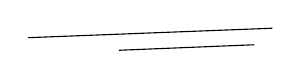
\begin{tikzpicture}[x=1cm,y=1cm]\draw (0,0) -- (3.1,.12);\draw (1.15,-.16) -- (2.87,-.09);\end{tikzpicture}}

\uline{Prouvons} f). Tout d'abord, comme les él. $\ne1$ de $H$ sont d'ordre $2$ et $3$, et que les élmts d'ordre $2$ sont contenus dans un sous-groupe inv. $V$ d'indice $2$, on voit que un syst. de Schwartz ne peut contenir deux él. d'ordre $2$, donc il contient au moins $2$ él. d'ordre $3$. \deleted{Soit $\rho,\rho',\unsure{\rho'|\rho''}$}

% archive sheet number: 50
\scanpage{52}

À \deleted{\unsure{symét}} op. près de $\unsure{\mathfrak S_3|\mathcal S_3}$, \unsure{SPS|PS|SS|OPS} donc que le système est de la forme $(\rho,\rho',\rho'')$, avec $\rho,\rho'$ d'ordre $3$, donc chacun de la forme $\rho_s$ ou $\rho_f$

\unsure{1)|A)} $\rho=\rho_f,\ \rho'=\rho_s$ il f. $s\prec f$ (car si $s$ opposé à $f$, $\rho_s=\rho_f^{-1}$ donc $\rho,\rho'$ n'engendrent pas $H$, donc on est dans le cas canonique

\margin{$12$}

\unsure{2)|B)} $\rho=\underset{\substack{\shortparallel\\\rho'_{f'}}}{\rho_s},\quad\rho'=\underset{\substack{\shortparallel\\\rho'_{s'}}}{\rho_f}$ il f. $s\unsure{\prec|\nprec} f$ i.e. $s'\prec f'$, donc on est dans le cas anticanonique

\margin{$12$}

3) $\rho=\rho_s,\ \rho'=\rho_{\deleted{\unsure{s'}}t}$ \inserted{$s,t\in S$} $(s\ne t)$ on est dans le \inserted{$1\textsuperscript{er}$} cas de e)

\margin{$12$}

4) $\rho=\underset{\substack{\shortparallel\\\rho'_{s'}}}{\rho_f},\quad\rho'=\underset{\substack{\shortparallel\\\rho'_{t'}}}{\rho_{\deleted{f'}g}}$ \inserted{$f,g\in F$} $(f\ne\deleted{f'}g)$ on est dans le $1\textsuperscript{er}$ cas de e)

\margin{$12$}

\uline{Corollaire} Les types numériques possibles des syst. de Schwartz pour $H\simeq\unsure{A_4|\mathcal A_4|\mathfrak A_4}$ sont

\[
\begin{aligned}
\text{a)}\ &(3,3,2)\ (3,2,3)\ (2,3,3)\qquad\text{[cas canonique et anticanonique]}\\
\text{b)}\ &(3,3,3)
\end{aligned}
\]

Et la classe de conjugaison sous $\widetilde H=\mathrm{Aut}_{\mathrm{gr}}(H)$. $(\simeq\mathfrak S_4)$ est déterminée par le type numérique.

Dans un $H$ $(\simeq A_4)$ un syst. de Schwartz est d'un des types suivants (où $H=\mathrm{Aut}^{+}(\Pi)$, $\Pi$ un tétraèdre comb., dont on n'a pas d'orientation privilégiée)

\margin{\uline{NB} La donnée de $H$ équivaut à celle de $\Pi$ cf plus haut}

a) On a un repère $r$ (\unsure{uniquemt|uniqmt|unique} déterminé) de $\Pi$, et $\Sigma=\Sigma_r$ (cas canonique)

\deleted{b) On a un \deleted{\unsure{orientation}} repère $r=\{s,\{s,s'\},\{s,s',s''\}\}$ bien déterminé et $\Sigma=(\rho_s^r,\rho_{s'}^r,\rho_{s''}^r)$, où l'exposant}

% archive sheet number: 51
\scanpage{53}

% archive sheet number: 52

\deleted{$r$ \inserted{\unsure{aux $\rho$}} indique que l'on utilise l'orientation définie par $r$ pour définir $\rho_s,\rho_{s'},\rho_{s''}$. \unsure{Une|Soit une} orientation \unsure{$\omega$} de $\Pi$, et une f.}

une suite (bien déterminée) $(s,s',s'')$ d'él. \unsure{distinct|distincts} de $S$, de sorte que, si $\omega$ est l'orientation de $\Pi$ \deleted{telle que la face} \inserted{qui \unsure{induit|induise} sur} la face $f=\{s,\unsure{s'|r'},s''\}$ l'orientation opposée de celle définie par l'ordre précédent, on ait

\[
\deleted{\unsure{\rho}}\Sigma=(\rho_s^\omega,\rho_{s'}^\omega,\rho_{s''}^\omega).
\]

[\uline{NB} la donnée de $s,s',s''$ équivaut à celle d'un repère, savoir $r=\{s,\{s\unsure{,|\mathord{\,}}s'\}\unsure{_s|{}},\{s,s',s''\}\}$].

\figure{\begin{tikzpicture}\draw (0,0) .. controls (1.3,-.65) and (2.2,-1.59) .. (3.75,-2.15);\end{tikzpicture}}

Cas de $\unsure{\mathfrak S_4|\mathcal S_4}$

\uline{Proposition} Soit $\Pi$ un octaèdre comb. \inserted{orienté}, et $H\inserted{=\mathrm{Aut}^{+}(\Pi)}$ le gpe de ses autom orientés, $R=\mathrm{Rep}\,(\Pi)$, $R^{+}=\mathrm{Rep}^{+}(\Pi)$

a) Pour tout $r\in R$, soit $\Sigma_r$ le syst. de Schwartz correspondant \inserted{de type $(\deleted{\unsure{4}}3,\deleted{\unsure{3}}4,2)$}. Alors $\Sigma_r=\Sigma_{r'}$ sss $r$ et $r'$ sont antipodiques, et l'ens des $\Sigma_r$ ($r\in R$) est égal à l'ens des $\Sigma_r$ ($r\in R^{+}$) et en corr. $1$--$1$ avec $R^{+}$ -- donc un torseur sous $H$.

\margin{$24$ d'où $6\times24=144$ \deleted{\unsure{NB}} syst. de Schwartz (en appliquant $\mathfrak S_3$)}

b) L'application $s\unsure{\longmapsto|\mathrel{\vdash\!\dashv}}\rho_s$ définit une bijection de $S$ avec $ {}_4H$ (ens des él. d'ordre $4$ de $H$)
\scanpage{54}

l'application $f\unsure{\mathrel{\vdash\!\dashv}|\longmapsto}\rho_f$ définit une bijection de $F$ avec $ {}_3H$, enfin l'application $a\mathrel{\vdash\!\dashv}\rho_a$ fait de $A$ un rev. de degré $2$ de \deleted{\unsure{$2$}} l'ens $ {}_2H\setminus {}_2H^{+}={}_2H^{-}$ (où $H^{+}=[H,H]\simeq\unsure{A_4|\mathcal A_4|\mathfrak A_4}$) formé des él d'ordre $2$ qui ne sont pas dans le ss-gpe invariant d'ordre $4$ de $H$ ; on a $\rho_a=\rho_{a'}$ \unsure{sss|ssi} $a,a'$ égaux ou antipodiques. Les applications $s\mathrel{\vdash\!\dashv}\rho_s$ et $f\mathrel{\vdash\!\dashv}\rho_f$ transforment antipodisme en passage à l'opposé $\rho\mathrel{\vdash\!\dashv}{\unsure{\rho|g}}^{-1}$.

c) Pour tout arc $(s,\deleted{\unsure{s'}}t)$ de $\Pi$, soit $f$ l'unique face telle que $(s,\{s,t\},f)\in R^{+}$. \deleted{un rep.} Alors

\[
(\rho_s,\rho_t,\rho_{f'})\qquad(f'\ \text{l'\uline{antipodique} de }f)
\]

est un syst. de Schwartz de type $(4,4,3)$. \inserted{L'ens \deleted{de}} Ces syst. de Schwartz forment un torseur sous $H$.

\margin{$24$ d'où $24\times3=72$ syst. de Schwartz en appliquant $\unsure{\mathfrak S_3|\mathcal S_3}$}

% slanted
\margin{\uline{NB} Un ss-gpe de $H=\mathfrak S_4$ qui est d'ordre multiple de $3$ et $4$, \unsure{ou|est} \unsure{soit|est} $H^{+}=A_5$, soit $H$ (or $\rho_s,\rho_t\notin H^{+}$ !)}

Si on regarde les \inserted{$6$} transformés de $(\rho_s,\rho_t,\rho_f)$ sous $\mathfrak S_3$, se groupent en couples de $2$ ayant $=$ caractère numérique, comme

\[
(\rho_s,\rho_t,\rho_f)\text{ et }
(\underset{\substack{\shortparallel\\\rho_{t'}}}{\rho_t^{-1}},
 \underset{\substack{\shortparallel\\\rho_{s'}}}{\rho_s^{-1}},
 \underset{\substack{\shortparallel\\\rho_{f'}}}{\rho_f^{-1}}),
\]

deux tels sont conjugués sous $H$ (en effet, $(t',\{t',s'\},f')\in R^{+}$ car l'antipodisme renverse l'orientation)

d) Les syst. de Schwartz énumérés épuisent tous les cas possibles.

% archive sheet number: 53
\scanpage{55}

\uline{Corollaire} Les types numériques possibles de syst. de Schwartz pour $H=\mathrm{Aut}^{+}(\Pi)$ sont les suivants

\[
\begin{aligned}
\text{a)}\ &(4,3,2)\ (3,2,4)\ (2,4,3)\ (2,3,4)\ (3,4,2)\ (4,2,3)\\
&\hspace{18em}\text{(canoniques)}\\
\text{b)}\ &(4,4,3)\ (4,3,4)\ (3,4,4)
\end{aligned}
\]

Le type numérique détermine le syst. de Schwartz modulo conjugaison. De façon précise, si $\Sigma=(\rho,\rho',\rho'')$ est un syst. de Schwartz, alors \unsure{elle|on|il} est dans l'un ou l'autre des cas suivants, s'excluant mutuellement

a) $\unsure{\exists\!\mid|\exists!|\exists}$ repère direct $r\in R^{+}$ \inserted{(unique)} tel que $\Sigma$ soit égal à $\Sigma_r$ ou un de ses transformé par $\sigma\in\unsure{\mathfrak S_3|\mathcal S_3}$ ($\sigma$ unique aussi)

b) $\exists\!\mid$ \deleted{arc \unsure{$s,t,f$}} $r\in R^{+}$, $r=(s,\{s,\deleted{\unsure{s'}}t\},f)$, \deleted{et} tel que $\Sigma$ soit égal à $(\rho_s,\rho_t,\rho_f)$ ou à un transformé par $\sigma\in\mathfrak S_3^{+}$ ($\sigma$ aussi unique).

\figure{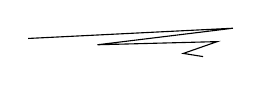
\begin{tikzpicture}\draw(0,0)--(2.6,.13)--(.88,-.08)--(2.4,-.04)--(1.97,-.19)--(2.22,-.23);\end{tikzpicture}}

Dém de d). Les ordres des él. $\ne1$ de $H$ sont $2,3,4$. Montrons d'abord qu'un système de Schwartz contient au moins un él. d'ordre $4$, et un \unsure{él|él.} d'ordre $3$.

% archive sheet number: 54
\scanpage{56}

$\rho=\rho_s,\ \rho'=\underset{\substack{\shortparallel\\\rho_{f'}^{-1}}}{\rho_f}$. Si $s\prec f$, on est dans le cas déjà traité dans a). Sinon, on a $s\prec f'$ donc

\deleted{\unsure{$\rho_s$} $(\rho_{f'},\rho_s,\rho_a)$ est un syst. de Schwartz canonique (où $a\in A$ est \unsure{choisi|défini} de façon que $(s,a,f')\in R^{+}$).}

\figure{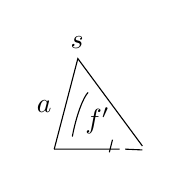
\begin{tikzpicture}[x=1cm,y=1cm]\draw(0,0)--(.30,1.15)--(1.12,.04);\draw(0,0)--(.83,0) (.9,0)--(1.12,-.01);\draw[thin](.70,-.04)--(.74,.12);\draw(.23,.16) .. controls (.28,.43) and (.37,.66) .. (.43,.72);\node[above] at (.29,1.15){$s$};\node[left] at (.09,.54){$a$};\node at (.55,.36){$f'$};\end{tikzpicture}}

\deleted{Donc $(\rho_s^{-1}\deleted{\unsure{^{2}}},\rho_{f'}^{-1}=\rho_f^{\deleted{\unsure{+}}},\rho_a^{-1}=\rho_a)=(\rho^{-1},\rho',\rho_a)$ est un syst. canonique. Donc \unsure{soit} $(\rho,\rho',\rho'')=\rho=\rho_s,\rho$}

Cela donne une seule autre possibilité comme position relative d'un él. d'ordre $4$ et d'un él. d'ordre $3$ qui ne commutent pas -- celui traité dans c) [type $(4,3,4)$] absurde. cqfd.

% archive sheet number: 55
\scanpage{57}

1) Il contient un él. d'ordre $4$, i.e. n'est pas formé d'él d'ordre $2$ et $3$.

Il \unsure{n'|ne} \deleted{est pas formé de} \inserted{peut contenir} deux él. d'ordre $2$, sinon $H$ serait un groupe diédral, ce qui n'est pas le cas. Donc il contiendrait deux él. d'ordre $3$, \deleted{\unsure{soit}} \inserted{qui engendrent $H$}

\deleted{$\rho_f,\rho_{\deleted{f'}g}$ $(f,g\in F)$ (\unsure{comme|jamais} $\rho,\rho'$ sont égaux ni opposés) On ne peut avoir \deleted{\unsure{$f=g'$}} $g=f$ ou $g=f'$, car $\rho_f,\rho_g$ \unsure{commuteraient}. Si on écrit $H\simeq\unsure{\mathfrak S_4|\mathcal S_4}$) $\pi_{123}$, et $\pi_{234}$ ou $\pi_{324}$ (modulo conjugaison) mais alors $\rho\rho'$ est}

\inserted{\unsure{or|ou}} les él. d'ordre $3$ sont dans $H^{+}$, absurde

2) Il contient aussi un él. d'ordre $3$, i.e. n'est pas formé \unsure{seult|seulmt|seulement} d'él. d'ordre $4$ et $2$. Car dans ce cas, comme il ne contient $2$ él. d'ordre $2$, il contiendrait au moins un autre él. d'ordre \deleted{\unsure{3}}$4$.

\deleted{Soient $\rho,\rho'$} \inserted{\unsure{SPS|Sps|OPS}} dans $(\rho,\rho',\rho'')$ que $\rho,\rho'$ sont d'ordre $4$ (quitte à utiliser $\mathfrak S_3$), donc de la forme $\rho_s,\rho_{\deleted{s'}t}$. \deleted{Mais \unsure{si}} \inserted{Évidt} \deleted{\unsure{a)}} $t\ne s,s'$ (antipodique de $s$), donc $(t,s)$ est un arc, on est dans le cas traité en c), où on a un él. d'ordre $3$.

3) Il reste (comme le cas de $2$ él. d'ordre $4$ est traité) à regarder le cas où on a un seul. él. d'ordre $4$, un d'ordre $3$, soit $(\rho,\rho',\rho'')$ avec

% archive sheet number: 56
